\documentclass[11pt]{article}
\usepackage[a4paper,margin=25mm]{geometry}
\usepackage[T1]{fontenc}
\usepackage{lmodern,microtype,amsmath,amssymb,graphicx,booktabs,tabularx,array,xcolor}
\usepackage{enumitem,caption,float,placeins}
\usepackage[colorlinks=true,linkcolor=teal!65!black,citecolor=teal!65!black,urlcolor=teal!65!black]{hyperref}
\usepackage{fancyhdr}
\setlength{\parskip}{5pt}
\setlength{\parindent}{0pt}
\setlength{\emergencystretch}{2em}
\setlist{nosep,leftmargin=1.5em}
\captionsetup{font=small,labelfont=bf}
\pagestyle{fancy}\fancyhf{}\fancyhead[L]{\small When Models Judge Models}\fancyhead[R]{\small Ramdowar}\fancyfoot[C]{\thepage}
\setlength{\headheight}{14pt}
\newcommand{\pp}{\,\mathrm{pp}}
\newcommand{\TV}{\operatorname{TV}}
\newcommand{\Neff}{N_{\mathrm{eff}}}
\title{\vspace{-1.2cm}\textbf{When Models Judge Models}\\[5pt]\large How Source Identity and Disagreement Shape\\Multi-Agent Financial Forecasts}
\author{Russlan Ramdowar\\\small Future Edge Group FZE, United Arab Emirates\\\small iPulse AI\\\small\href{mailto:russlan@ipulseai.com}{russlan@ipulseai.com}\\\small ORCID: \href{https://orcid.org/0009-0004-9311-6957}{0009-0004-9311-6957}}
\date{1 October 2026}
\begin{document}
\maketitle
\begin{abstract}
The same research reports can support a predicted gain or a predicted loss, depending on which AI combines them. We examine this decision layer in a seven-asset case study from iPulse AI's investment-research pipeline. For each asset, we hold fourteen reports and their forecasts fixed. Instead of simply averaging the forecasts, an AI synthesizer judges each report's influence; code applies its weights. We compare two synthesizers, repeat their judgments, reverse the report order, and reveal the source models. Switching from Gemini to Astra reverses the direction of the five-year forecast for two of six equities; for Bitcoin, the forecasts differ by 29.45 percentage points. Revealing the source models also raises Astra's allocation to its own report in every equity, without a comparable increase for the Opus report. This pattern is consistent with selective preference, but does not establish its cause. Our central finding is that agreement among the inputs, stability of the weights, and stability of the final forecast are distinct properties. The study makes each step inspectable through released reports, weights, rationales, and calculation code. It evaluates how AI systems combine evidence, not whether their predictions are correct: the forecasts have not yet matured.
\end{abstract}
\textbf{Keywords:} multi-agent systems; language-model evaluation; forecast aggregation; source identity; robustness; financial research.

\section{The same evidence, a different final answer}
Fourteen reports about Moderna enter a synthesis pipeline. Under one synthesizer, the resulting five-year price forecast is $+4.98\%$. Under another, it is $-9.98\%$. The underlying reports and their forecast paths are unchanged. What changes is the allocation of influence.

The architecture resembles a \emph{research council}: advisor configurations submit separate reports, a synthesizer assesses them, and code converts their assigned influence into a forecast. Equal-report averaging gives every report the same weight, without judging its evidence or reasoning. Synthesis can instead respond to the substance of disagreement, but adds another model-dependent decision. It must earn any advantage over averaging through evaluation. The council is an analogy for this division of work, not an iterative debate among agents.

The setting is iPulse AI's regular deep-analysis pipeline. Its completed Batch 7 release, audited on 21 September 2026, covers 426 curated assets, with fourteen source opinions and one consensus per asset: 5,964 reports and 426 consensuses. Figure~\ref{fig:design} shows how this paper branches from that workflow. We reuse seven assets' reports generated on 20 September 2026, holding their content and forecast paths fixed while changing the synthesizer, report order, or source-model disclosure.

\begin{figure}[!t]
\centering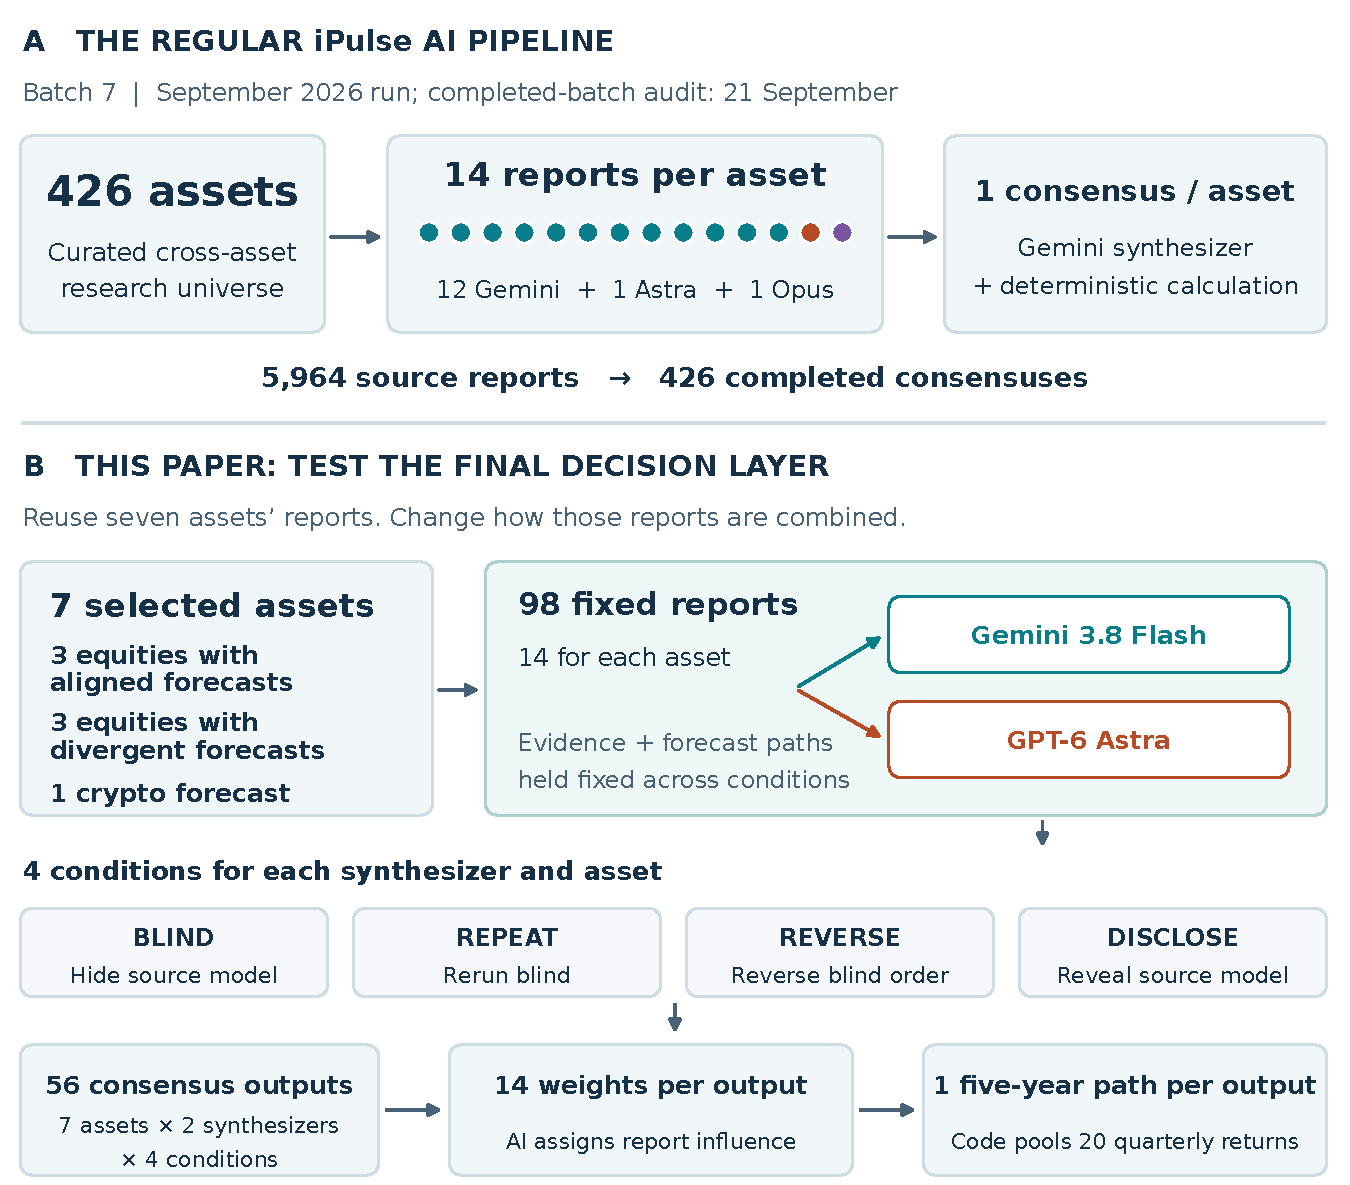
\includegraphics[width=\linewidth]{figures/design.pdf}
\caption{From the production pipeline to the fixed-report experiment. Each dot in panel A represents one source report, not an independent model. Panel B reuses three aligned equities, three divergent equities, and Bitcoin: $7\times14=98$ reports and $7\times2\times4=56$ consensus outputs. Seven original Gemini baselines are reused; the remaining 49 outputs are new requests. The four conditions change presentation or source labels; cross-synthesizer comparisons also differ in execution and retrieval. Bitcoin's reversal and disclosure conditions additionally change a checklist, so matched treatment comparisons use the six equities. Arrows show workflow, not learned neural connections or measured weights.}
\label{fig:design}
\end{figure}

This design connects to an established line of work on models combining other models' outputs: LLM-Blender ranks and fuses candidate responses~\cite{blender}, while Mixture-of-Agents uses layered aggregation~\cite{moa}. Self-MoA shows why mixing more model families does not automatically improve results~\cite{selfmoa}. Our contribution is to expose this decision layer in an operational forecasting workflow, with explicit weights, simple averaging comparators, and inspectable numerical consequences.

\begin{samepage}
The practical stakes come from repeated deployment. The completed-release records account for 643.3 million input tokens and 141.2 million generated tokens, including reasoning, across 6,816 recorded generation stages (Appendix~\ref{app:resources}). These counts describe workload, not research quality. They make the operational question concrete: after substantial effort has produced different perspectives, how does the final layer decide which perspectives count?
\end{samepage}

We examine that transition in iPulse AI's Batch 7 archive. The system separates \emph{semantic synthesis} from \emph{arithmetic}: a language model evaluates fourteen reports and emits a weight for each; code normalizes the weights, averages each quarter's forecasted return, and compounds the resulting path. This separation makes the last stage inspectable. We can ask who receives influence, whether that influence changes when names or order change, and how much the resulting forecast moves.

The paper studies three connected questions. First, how much does changing the synthesizer change the result? Second, does revealing the model behind a report shift its weight, including toward the synthesizer's own family? Third, when does a change in weights become a large change in the forecast? The third question prevents a common shortcut: treating a stable weight vector as equivalent to a stable decision, or a changed weight vector as necessarily consequential.

Our contribution is an auditable case study of this full pathway, not a new claim that language-model judges can be biased. The archive includes the complete source reports supplied to synthesis, original request content, normalized and submitted weights, written rationales, and all forecast steps. Deterministic reproduction shows precisely where the two deployed synthesizers differ. An elementary sensitivity bound explains why disagreement matters. Simple alternative pooling rules reveal that even the arithmetic definition of consensus can change the sign of a forecast.

The strongest conclusions concern \emph{system behavior}. Neither apparent sophistication nor repeatability establishes accuracy. The first forecast targets are in December 2026, after this paper's cutoff. No result here demonstrates investment performance, a superior model, or an unbiased source-quality ranking.


\section{Position in the literature}
\textbf{Aggregation is a modeling choice.} Forecast combination has a long history: Bates and Granger~\cite{bates} estimated combinations using past forecast errors. Here, weights instead arise from a language model's assessment of evidence and reasoning before outcomes are available. They are neither estimated accuracy weights nor posterior model probabilities. Recent language-model ensembles rank and fuse responses~\cite{blender} or aggregate outputs across layers of agents~\cite{moa}; work questioning the benefit of model diversity shows why more model families cannot simply be assumed to improve an ensemble~\cite{selfmoa}. Our setting exposes continuous report-level influence and its deterministic downstream consequences.

\textbf{Judges are sensitive to more than content.} LLM-as-a-judge research documents evaluation limitations~\cite{mtbench}, self-recognition and self-preference~\cite{panickssery}, and familiarity-related preference~\cite{wataoka}. Position and presentation also matter~\cite{fair,sclar}, while long-context studies show that access to information is not equivalent to reliable use of it~\cite{lostmiddle}. These findings motivate the repeat, reversal, and disclosure conditions. They do not establish the mechanism of any change in our archive: source reports differ in quality and style, retrieval is not fixed, and true labels are not randomly reassigned.

\textbf{Robustness is not forecast skill.} A convincing rationale is not a verified explanation of a model's internal decision process~\cite{turpin}. Likewise, a robust point forecast is not automatically accurate. ForecastBench illustrates prospective evaluation using unresolved questions~\cite{forecastbench}; point-forecast evaluation requires an explicit target and scoring function~\cite{gneiting}. We therefore treat the present release as a study of aggregation behavior. A later, separately specified outcome study must test forecast skill.

\section{Archive, sample, and experimental design}
\subsection{What is held fixed}
For each asset, fourteen reports supply investment frameworks, evidence references, narrative assessments, and twenty quarterly price-return predictions. Twelve reports are attributed to Gemini 3.8 Flash, one to Claude Opus 5, and one to GPT-6 Astra. The latter two use the Universal Investor framework; the twelve Gemini reports span additional frameworks and modes. The source composition is intentionally unbalanced and does not constitute fourteen independent model families.

We use the model names and deployment identifiers recorded in the archive: \texttt{gemini-3.8-flash} and \texttt{gpt-6-astra} for the synthesizers. These labels identify the archived executions, not independently established capability tiers. For readability, the text subsequently uses \emph{Gemini} and \emph{Astra}; \emph{Opus} refers to the source report, not a third synthesizer.

The archived source reports were generated on 20 September 2026. Source evidence and twenty-step paths are fixed within each asset across conditions. Equities use an 18 September anchor, Bitcoin a 20 September anchor. SAP is the Xetra listing, in euros. These are price-path forecasts; they do not include dividends, trading costs, or portfolio rebalancing returns. Individual period predictions are called ``most reasonable'' in the source schema. That label does not establish that they are conditional expectations, medians, or draws from a calibrated predictive distribution.

\subsection{Framework, mode, and model are different design choices}
A source opinion is defined by three distinct choices. Its \emph{framework} determines the investment questions and causal lens: for example, ownership economics, political power, or technological disruption. Its \emph{mode} determines evidence acquisition: \emph{Thinker} reasons from supplied, dated context without live search; \emph{Researcher} can search for evidence needed to support or challenge the thesis. Its \emph{model} is the language-model implementation carrying out that work. Reports also contain shared context and configured presentation instructions; framework and mode are not the only possible sources of difference.

The fourteen-opinion recipe crosses these choices selectively, not factorially. Gemini supplies one Researcher report for each of nine frameworks, plus Thinker variants for Value Ownership, Civilizational Compute, and Universal Investor. Astra and Opus each add a Universal Investor Researcher report. Thus, \textbf{twelve Gemini opinions represent framework and mode diversity within one model family}, while the Universal Investor Researcher configuration provides a narrower three-model comparison. This operational recipe explains the unequal counts; it is not evidence that twelve independent models agree, nor was it chosen here as a balanced model-ranking design.

\begin{table}[H]
\centering\small
\begin{tabularx}{\linewidth}{@{}>{\raggedright\arraybackslash}p{.27\linewidth}>{\raggedright\arraybackslash}X >{\raggedright\arraybackslash}p{.17\linewidth}@{}}
\toprule
Framework / archetype & Investment lens & Source recipe \\
\midrule
Value Ownership / Buffett & Business quality, durable moats, owner cash flows, and margin of safety. & Gemini R + T \\
Economic Machine / Dalio & Debt cycles, liquidity, policy regimes, and macroeconomic cause and effect. & Gemini R \\
Paradigm Shift / Visionary & First-principles feasibility, adoption curves, execution, and technological disruption. & Gemini R \\
Empire Dominance / Titan & Pricing power, strategic bottlenecks, consolidation, and regulatory counterpressure. & Gemini R \\
Power Audit / Insider & Political influence, institutional incentives, policy exposure, and protection. & Gemini R \\
Contrarian / Vulture & Mispricing, stressed fundamentals, overlooked risks, and catalysts that challenge consensus. & Gemini R \\
Forensic Deduction / Whistleblower & Accounting quality, missing evidence, contradictions, and verifiable claims. & Gemini R \\
Civilizational Compute / Anthropologist & Long-run needs, resource efficiency, information networks, and technological displacement. & Gemini R + T \\
Universal Investor / Polymath & Integrates the other lenses and identifies which forces matter most for the asset. & Gemini R + T; Astra R; Opus R \\
\bottomrule
\end{tabularx}
\caption{Nine framework families generate fourteen opinions per asset. R denotes Researcher and T denotes Thinker. Names are mnemonic AI configurations, not reports by or endorsements from their namesakes. Descriptions summarize the platform's persona definitions; the companion data maps all 98 archived reports to framework, mode, and model.}
\label{tab:frameworks}
\end{table}

\subsection{Seven assets, with two different roles}
The archived protocol describes 189 eligible equities with the required source composition and twenty parsed steps. It combines terminal sign agreement, average quarterly sign agreement, and the cross-sectional percentile of terminal-return interquartile range (IQR) into consistency and dispersion scores. It selects three large-capitalization assets from each top-ten list, using recorded market-capitalization snapshots as a recognition proxy. Visa, SAP, and IBM form the directionally consistent cohort; Nebius, Moderna, and Kratos form the dispersed cohort. Bitcoin is a fixed crypto reference.

This is deliberate case selection, not a random market sample. We preserve the recorded procedure and the selected reports, but the complete 189-asset ranking input is not recovered in this release. Consequently, the selection ranking and market-cap snapshots are documented provenance, not independently reproduced sample-selection results. Cohort differences should not be interpreted as population estimates.

The initial predictions make the intended contrast visible. Every report predicts a positive five-year return for Visa, SAP, and IBM. Nebius and Moderna each divide seven positive against seven negative forecasts; Kratos divides eight against six. Bitcoin is a different kind of disagreement: all fourteen terminal returns are positive, but their magnitudes vary widely. The design is therefore \textbf{three aligned equities, three divergent equities, and one crypto reference}, not four equities selected under the dispersion rule. Treating Bitcoin as simply a fourth divergent asset would hide the distinction between disagreement about direction and disagreement about magnitude.

\begin{table}[ht]
\centering\small
\begin{tabular}{@{}llrrr@{}}
\toprule
Recorded group & Asset & Positive & Negative & Terminal IQR (pp) \\
\midrule
Aligned equities & Visa & 14 & 0 & 7.99 \\
& SAP & 14 & 0 & 17.38 \\
& IBM & 14 & 0 & 11.70 \\
\addlinespace
Divergent equities & Nebius & 7 & 7 & 78.95 \\
& Moderna & 7 & 7 & 81.66 \\
& Kratos & 8 & 6 & 84.97 \\
\addlinespace
Crypto reference & Bitcoin & 14 & 0 & 64.33 \\
\bottomrule
\end{tabular}
\caption{Disagreement in the fourteen \emph{initial source forecasts}, before either synthesizer allocates weights. Positive and negative count five-year cumulative price returns; none is zero. The selected-source diagnostics are independently recomputed, while the full original ranking universe remains unavailable.}
\label{tab:initial}
\end{table}

The broader operational release is also distinct from the experiment. A recovered closure ledger reconciles 426 asset syntheses and 5,964 distinct successful source-task identifiers: 383 equities, 19 cryptocurrencies, 14 forex instruments, five commodities, and five indices. That is 6,390 logical tasks, not a count of API attempts or billable executions. Our comparative evidence remains seven assets and 56 outputs.

\subsection{Historical context and the original forecast paths}\label{sec:history}
We show each asset's five-year price history, sampled weekly from the platform's BigQuery records together with all fourteen initial forecast paths, both original blinded consensus paths, and an equal-report comparator in Appendix~\ref{app:history}. The charts use price units and the exact archived anchor rather than replacing the starting price with an index. This allows readers to see the market-price context leading into the forecast and then inspect the range of alternative futures from the same starting point. No initial report is hidden merely because a synthesizer gives it little weight.

The history uses 8,711 daily stored closes retrieved from BigQuery on 1 October 2026, reduced to 1,689 weekly observations. We take the last available close in each Monday--Sunday week, keep its actual date, and include the final partial week. Each chart spans five years before and five years after its frozen anchor, so history and forecasts occupy equal horizontal widths. The six equity anchor-date closes match their archived anchors exactly; Bitcoin history stops on 19 September, before its 20 September 00:00 UTC anchor. Missing currency fields are resolved from the asset dimension and checked against the frozen inputs.

No line is drawn across gaps longer than fourteen days. Nebius includes predecessor Yandex observations. \href{https://ir.nasdaq.com/news-releases/news-release-details/nasdaq-resumes-trading-nebius-group-nv}{Nasdaq records a trading halt from 28 February 2022 until 21 October 2024}; the chart labels the suspension explicitly. We plot the stored \texttt{close} field without local adjustment or rescaling. Daily close timestamps are absent, and vendor adjustment conventions are not independently reconstructed. The release documents the extraction and sampling procedure. Historical price CSVs are not redistributed; recreating the historical chart backgrounds requires independently authorized price data. All frozen forecast paths and the core comparison results are included and reproducible offline. This is retrospective context, not a point-in-time data vintage, extra model input, or forecast-outcome test. Cohorts were selected from forecast disagreement, not these historical paths.

\subsection{Two synthesizers, four conditions}
\begin{table}[ht]
\centering\small
\begin{tabularx}{\linewidth}{@{}lXX@{}}
\toprule
Condition & Presentation & Execution count \\
\midrule
Blinded baseline & Canonical report order; source model labels withheld & 7 reused Gemini outputs; 7 new Astra outputs \\
Blinded repeat & Same presentation as baseline & 7 new outputs per synthesizer \\
Reversed order & Report order reversed; associated checklist order follows it & 7 new outputs per synthesizer \\
Model disclosed & Canonical order; true source-model labels supplied & 7 new outputs per synthesizer \\
\bottomrule
\end{tabularx}
\caption{There are 49 newly executed synthesis requests and seven reused Gemini baselines, giving 56 outputs. Only two blinded realizations exist per asset and synthesizer; reversal and disclosure each have one.}
\label{tab:design}
\end{table}

The archived Gemini settings use temperature 0.2 and a 65,536-token output/thinking ceiling. Astra uses high reasoning and a 65,536-token output ceiling. Both have web-search tools available. Their matched experimental requests contain the same system and user content, but provider schemas, reasoning controls, tools, and execution times differ. Cross-synthesizer comparisons therefore compare deployed systems, not isolated model architectures.

Disclosure adds a source-model field and changes the instruction explaining whether identities are withheld or supplied. The prompt still asks for judgment based on evidence and causal reasoning rather than prestige. Blinding removes explicit source labels, not every possible stylistic cue. Reversal changes the full presentation order, including the report-ID checklist; it is not a clean estimate of one positional mechanism.

\textbf{The Bitcoin qualification matters.} A prompt audit found an additional checklist in Bitcoin's reverse-order and disclosed conditions relative to its baseline and repeat. We therefore report the six equities as the matched treatment panel and describe Bitcoin's treatment results separately. This exclusion is an audit-driven analytical decision, not a prospectively registered exclusion. Bitcoin remains fully included in the baseline synthesizer comparison and the seven-asset path display. Its baseline comparison is the largest in the panel.

The internal protocol predates the saved experimental results according to the local workflow, but an independent public registration timestamp has not been established. We call it an \emph{archived protocol}, not an externally verified preregistration. No new model inference was performed to prepare this paper.

\section{From influence to a forecast}
\subsection{The pooling operator}
Let $r_{it}$ be report $i$'s predicted return in quarter $t$, expressed as a decimal, with $i=1,\ldots,14$ and $t=1,\ldots,20$. The synthesizer submits nonnegative scores $s_i$ with positive total. Code normalizes them to weights $w_i=s_i/\sum_j s_j$. A single weight vector applies to all twenty quarters:
\begin{equation}
q_t(w)=\sum_i w_i r_{it},\qquad
R_T(w)=\prod_{t=1}^{T}\bigl(1+q_t(w)\bigr)-1.
\label{eq:step}
\end{equation}
The price path is $P_T=P_0[1+R_T(w)]$. The report rationales are not additional numerical inputs after the weights have been emitted. We recompute every quarter and cumulative return from the saved weights and source matrix. The archive normalizes to twelve decimal places with a residual adjustment; the independent implementation verifies the resulting simplex and paths within numerical tolerances.

Pooling each quarter and then compounding is not the same operation as pooling complete paths:
\begin{equation}
\widetilde R_T(w)=\sum_i w_i\left[\prod_{t=1}^{T}(1+r_{it})-1\right].
\label{eq:path}
\end{equation}
Neither expression is automatically the correct expectation of future prices. Equation~\ref{eq:step} is the deployed operator we audit; Equation~\ref{eq:path} is a deterministic sensitivity check. They answer different aggregation questions.

\subsection{Three quantities that should not be conflated}
We report weight movement as total variation, $\TV(w,v)=\frac12\sum_i|w_i-v_i|$. A value of 0.10 means that ten percent of total influence must be reallocated to transform one normalized vector into the other. Concentration is summarized by $\Neff=1/\sum_iw_i^2$. This is an effective number of equally weighted reports, not a count of independent information sources. Output movement is the absolute difference in the one-year or five-year compounded return, in percentage points.

These quantities interact through the source forecasts. For every quarter,
\begin{equation}
|q_t(w)-q_t(v)|\leq \TV(w,v)\left(\max_i r_{it}-\min_i r_{it}\right).
\label{eq:bound}
\end{equation}
This elementary bound follows by moving at most $\TV(w,v)$ mass between the smallest and largest values; it is not a new theorem. If all reports agree numerically, changing their weights cannot change that quarter's return. When they disagree, where the weight moves matters as well as how far it moves. Compounding adds dependence on the full sequence of quarterly returns. Terminal IQR is a readable description of source dispersion, not a substitute for the per-quarter range in Equation~\ref{eq:bound}.

We use paired, descriptive comparisons within each asset. The experimental unit is the asset, not each of its fourteen weights or twenty forecast steps. With six selected equities, one reversal, and one disclosure realization per synthesizer, significance tests and narrow confidence intervals would convey unwarranted precision. We report each asset and the simple cohort means instead.

\section{Results}
\subsection{Changing the synthesizer changes the forecast's direction}
\begin{figure}[t]
\centering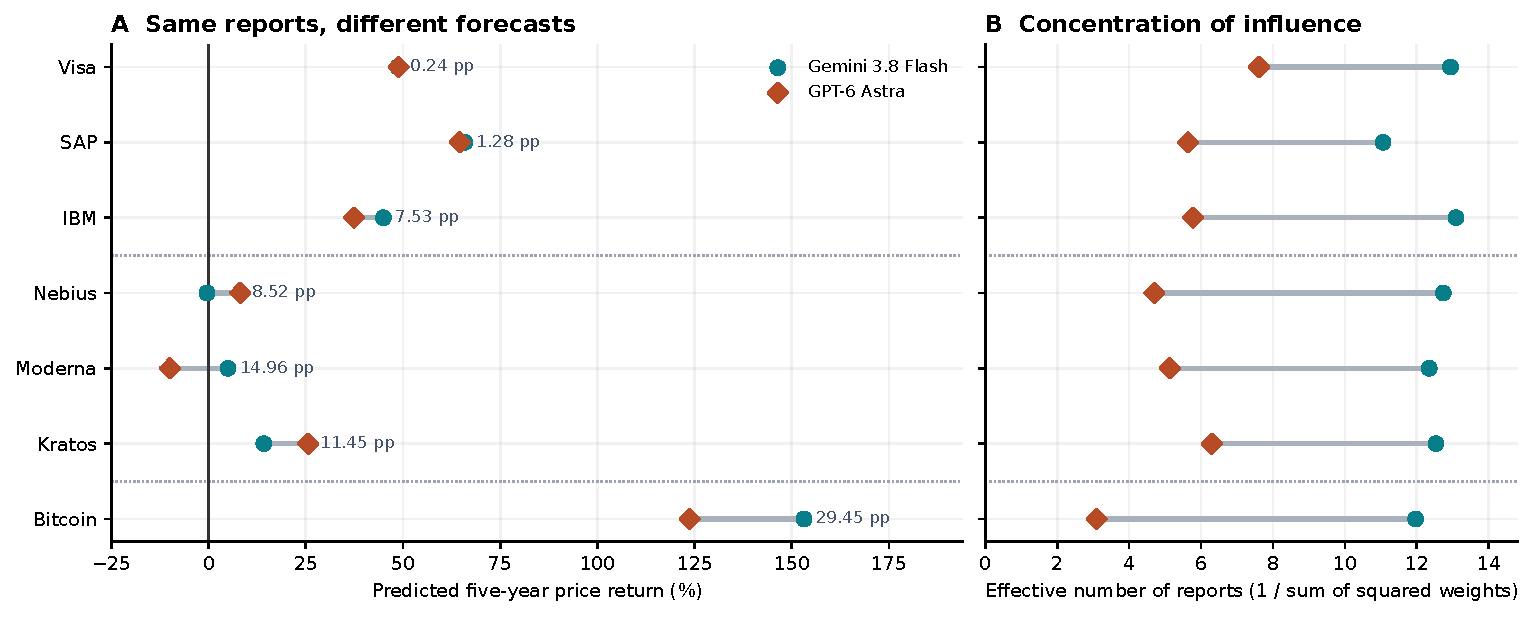
\includegraphics[width=\linewidth]{figures/synthesizer_choice.pdf}
\caption{Blinded baselines for all seven assets. Left: predicted five-year returns; annotations give the absolute between-synthesizer gap. Right: effective number of reports. Dotted horizontal lines separate the two equity cohorts and Bitcoin. Both panels describe archived allocations and predictions, not realized accuracy.}
\label{fig:choice}
\end{figure}

Figure~\ref{fig:choice} shows that synthesizer choice is numerically consequential even with the source reports fixed. Nebius moves from $-0.42\%$ under Gemini to $+8.10\%$ under Astra; Moderna moves from $+4.98\%$ to $-9.98\%$. These are five-year sign reversals, not classifications inferred from prose. Kratos remains positive but moves from $14.19\%$ to $25.64\%$.

For Visa, SAP, and IBM, the mean absolute five-year gap is 3.02 percentage points. For Nebius, Moderna, and Kratos it is 11.64 points, or 3.86 times as large. The comparison is consistent with the role of source disagreement, but it does not isolate disagreement causally: cohorts differ in companies, narratives, and forecast matrices. Nor are aligned assets immune; IBM's gap is 7.53 points. The corresponding Visa gap is only 0.24 points despite a weight-TV distance of 0.244. Allocation difference and numerical difference are plainly not interchangeable.

Figure~\ref{fig:dispersion} connects the initial source disagreement directly to the synthesizer comparison. The three divergent equities have terminal source IQRs near 79--85 points, compared with 8--17 points for the aligned equities. Their larger typical synthesis gaps are therefore interpretable against the alternatives available to the synthesizer. The relationship is not monotonic: Bitcoin has a smaller IQR than the divergent equities but the largest synthesis gap. Dispersion describes the available disagreement; the location and size of weight transfers determine which part of it reaches the final forecast.

\begin{figure}[ht]
\centering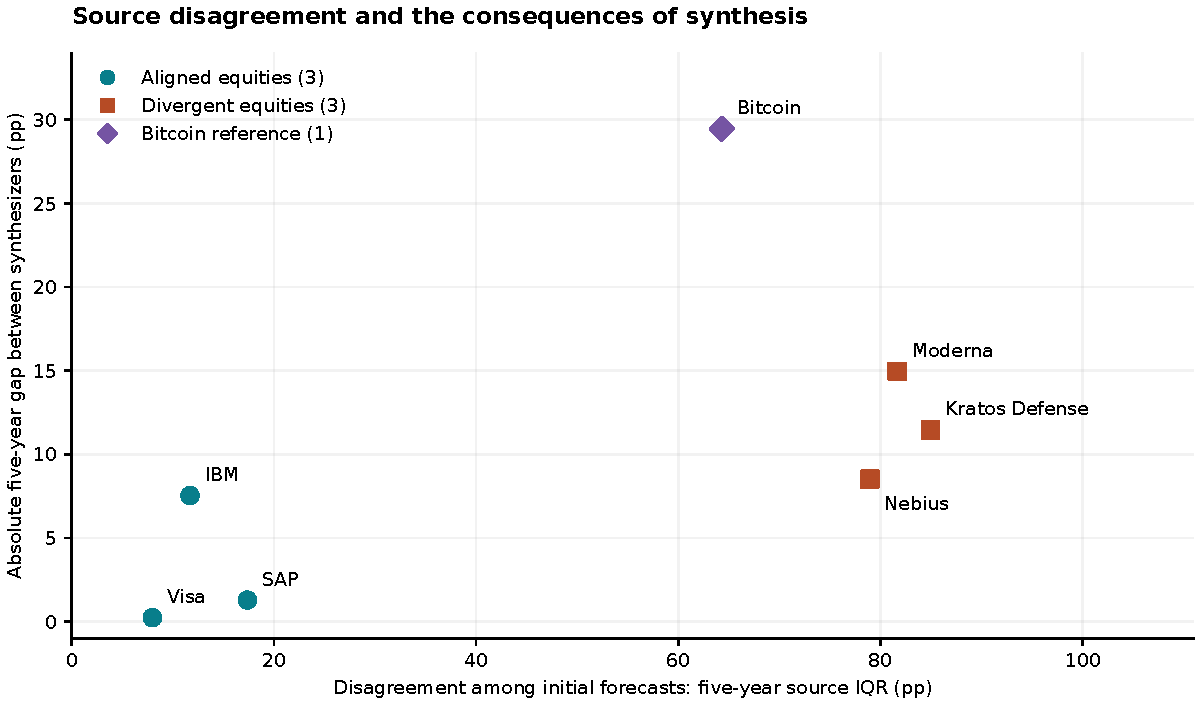
\includegraphics[width=.94\linewidth]{figures/dispersion_vs_synthesis.pdf}
\caption{The comparison begins with the initial predictions. Each point is one asset: source-return dispersion on the horizontal axis, and the absolute five-year gap between the two blinded consensus baselines on the vertical axis. Cohort membership is the recorded selection, not a grouping fitted to these outcomes. Seven selected cases do not establish a population regression or a causal effect of dispersion.}
\label{fig:dispersion}
\end{figure}

Across the six equity baselines, mean effective report count is 12.45 for Gemini and 5.86 for Astra. Astra makes more concentrated judgments. That may reflect selective use of evidence, excessive deference to a few reports, or both; concentration itself cannot distinguish them. It is not evidence that Astra is more accurate or that Gemini is appropriately diversified.

\begin{table}[ht]
\centering\small
\begin{tabular}{@{}lrrrrr@{}}
\toprule
& \multicolumn{2}{c}{One-year return (\%)} & \multicolumn{2}{c}{Five-year return (\%)} & Source IQR \\
Asset & Gemini & Astra & Gemini & Astra & (five-year pp) \\
\midrule
Visa & 6.66 & 5.76 & 48.68 & 48.92 & 7.99 \\
SAP & 11.57 & 10.13 & 65.88 & 64.60 & 17.38 \\
IBM & 6.60 & 4.58 & 44.96 & 37.43 & 11.70 \\
Nebius & -10.62 & -5.33 & -0.42 & 8.10 & 78.95 \\
Moderna & -23.60 & -21.42 & 4.98 & -9.98 & 81.66 \\
Kratos & -3.73 & -2.30 & 14.19 & 25.64 & 84.97 \\
Bitcoin & 18.52 & 10.51 & 153.15 & 123.70 & 64.33 \\
\bottomrule
\end{tabular}
\caption{Blinded baseline predictions and disagreement among the fourteen source paths. One year means four forecast steps; five years means twenty. Returns are cumulative price returns, not annualized or realized returns.}
\label{tab:assets}
\end{table}

\subsection{Bitcoin: agreement about direction is not agreement about magnitude}
All fourteen Bitcoin reports predict a positive five-year return, yet their middle fifty percent spans 64.33 percentage points. This is much wider than the middle ranges in the aligned equity cohort. The two synthesizers predict $153.15\%$ and $123.70\%$: a 29.45-point gap, larger than for any equity in the panel.

Astra allocates 55\% of Bitcoin's baseline weight to its own source report; Gemini allocates 12.86\% to that same report. Their effective report counts are 3.10 and 11.97. Positive sign agreement therefore does not mean that aggregation choices are harmless. A decision-maker can face a large difference in predicted upside even when no report predicts a loss.

Bitcoin also limits broad claims about repeatability. Its five-year same-order repeat difference is 1.97 points for Astra and 1.83 for Gemini, reversing their equity-level ordering on this measure. In the confounded disclosure condition, Astra's own-source weight falls from 55\% to 52\%. We retain this contrary observation rather than generalizing the six-equity pattern to all seven assets.

\subsection{Disclosure shifts influence selectively}
\begin{figure}[t]
\centering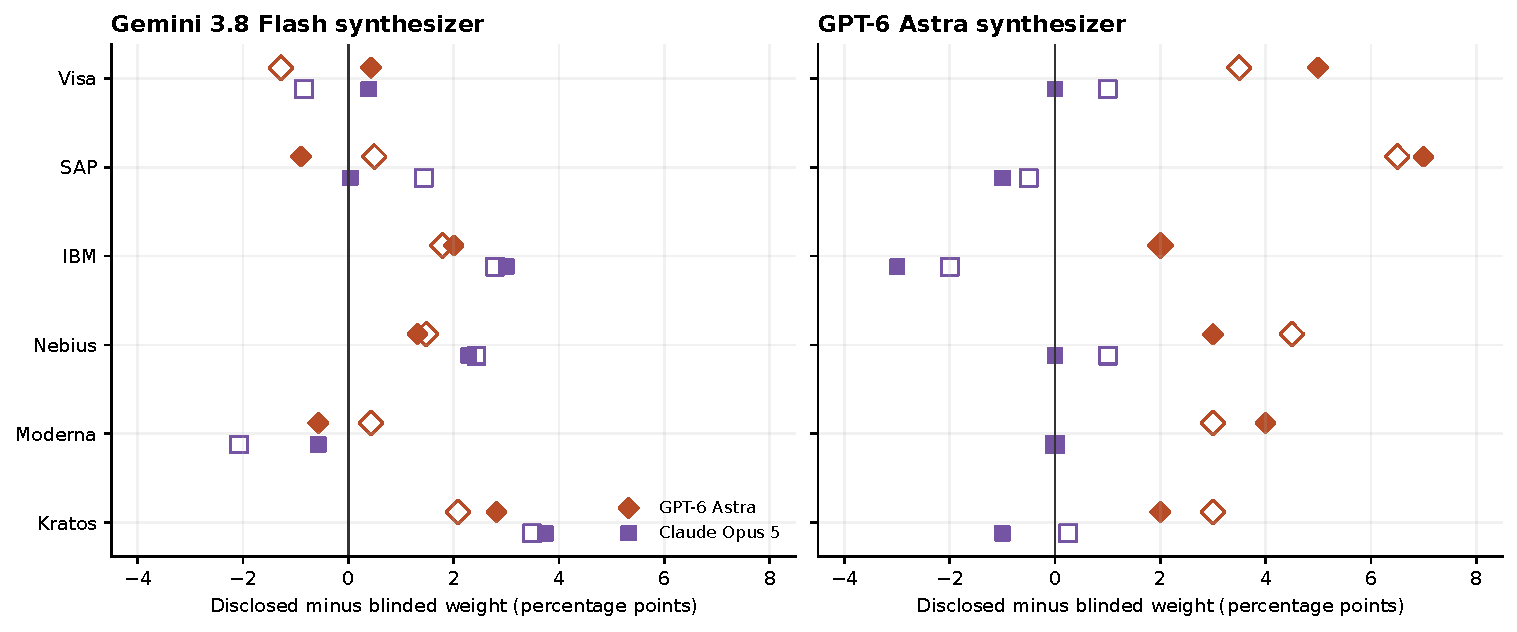
\includegraphics[width=\linewidth]{figures/source_disclosure.pdf}
\caption{Source-model disclosure in the six matched equities. Filled markers compare the disclosed run with the original blinded baseline; hollow markers compare it with the mean weight of the two blinded runs. Diamonds identify the Astra source report; squares identify the Opus source report. Each is one of fourteen reports. The two reference choices reveal why Astra's own-source uplift is more consistent than an Opus penalty.}
\label{fig:disclosure}
\end{figure}

Under Astra synthesis, revealing source identities increases the Astra report's weight in all six equities: $+5$, $+7$, $+2$, $+3$, $+4$, and $+2$ percentage points for Visa, SAP, IBM, Nebius, Moderna, and Kratos, respectively. The mean increase is $+3.83$ points, from a mean baseline weight of 33.67\% to 37.50\%. The mean change for the Opus report is $-0.83$ points. Under Gemini synthesis, the Astra and Opus reports instead gain $+0.85$ and $+1.48$ points on average (Table~\ref{tab:disclosure}).

The blinded repeat provides a necessary qualification. Comparing disclosure with the mean of the two blinded runs leaves Astra's own-source uplift nearly unchanged at $+3.75$ points, but reduces the mean Opus change to $-0.04$ points. The defensible description is \emph{selective own-source uplift in this equity panel}, not a robust penalty against Opus. The baseline-referenced difference between the Astra and Opus changes is $+4.67$ points.

\begin{table}[ht]
\centering\small
\begin{tabular}{@{}llrr@{}}
\toprule
Synthesizer & Source group & Versus original blind & Versus mean of two blinds \\
\midrule
Gemini & Astra (one report) & +0.85 & +0.83 \\
Gemini & Opus (one report) & +1.48 & +1.21 \\
Gemini & Gemini (twelve reports) & -2.33 & -2.04 \\
\addlinespace
Astra & Astra (one report) & +3.83 & +3.75 \\
Astra & Opus (one report) & -0.83 & -0.04 \\
Astra & Gemini (twelve reports) & -3.00 & -3.71 \\
\bottomrule
\end{tabular}
\caption{Mean change in total normalized source-group weight, in percentage points, across six equities. The Gemini row aggregates twelve reports and is not directly comparable to a single report's weight; its original-blind per-report changes are $-0.19$ points under Gemini synthesis and $-0.25$ under Astra. Within each synthesizer and reference, group changes sum to zero before rounding.}
\label{tab:disclosure}
\end{table}

The allocation pattern is compatible with source-identity preference, but it does not identify self-preference as its cause. Disclosure conveys true information, source reports differ, provider retrieval may vary, and there is only one disclosed realization. The Opus report is a useful outside-family comparator, not a randomized quality-matched control. It sharpens the question: does disclosure reward any alternative to Gemini, or specifically the synthesizer's own source? Astra's own-source uplift persists against both blinded references, whereas Opus has essentially no mean uplift against the two-blind reference. This is a selective pattern, rather than a uniform premium for both minority-model reports.

\textbf{A shared framework strengthens the comparison, but does not settle the mechanism.} The Astra and Opus reports both use Universal Investor in Researcher mode. The same framework and mode are also available under Gemini. In this narrower three-report comparison, Astra synthesis changes the Gemini report's weight by $-0.50$ points, its own report by $+3.75$, and Opus by $-0.04$, relative to the mean of two blinded runs. Under Gemini synthesis, the corresponding changes are $-0.58$, $+0.83$, and $+1.21$. The pattern is therefore not symmetric family favoritism across both synthesizers. These are absolute weights in the original fourteen-report ensemble, not a rerun using only three reports.

Even comparable performance on an external benchmark would not show that two particular investment reports have equal quality. The models can differ in relevant evidence, retrieval, factual reliability, argument structure, or perceived expertise on this task. Their identities may also carry task-specific reputation priors. This archive has neither independent report-quality labels nor a matched benchmark establishing that these exact deployments are equally capable. Opus therefore strengthens the \emph{diagnostic contrast}; it does not prove that Astra's uplift is unjustified, conscious, or caused by self-recognition. A label-swap experiment holding the text fixed, with repeated draws and fixed retrieval, would better separate a name effect from legitimate evidence assessment. This archive does not contain that experiment.

\subsection{Repeatability does not imply order robustness}
Across the six equities, Astra's mean same-order TV distance is 0.0475, compared with 0.0830 for Gemini: 42.8\% less movement in this descriptive average. Its mean absolute five-year repeat difference is 0.93 rather than 2.17 percentage points, 57.2\% lower. These observations support greater same-order repeatability in this panel, not a universal robustness ranking.

Reversing report order changes the picture. Mean TV is similar---0.1008 for Astra and 0.1045 for Gemini---but Astra's mean absolute five-year movement is larger: 2.04 versus 1.37 points. The same model can look more stable under one perturbation and less stable under another. A single robustness score would hide that distinction (Figure~\ref{fig:stability}).

Disclosure also illustrates the gap between an interesting allocation effect and a large terminal effect. The own-source shift under Astra coexists with a mean absolute five-year movement of only 0.79 points, smaller than its 2.04-point reversal movement. Weight changes must be traced through the particular forecasts they reweight; their rhetorical significance is not a measure of their numerical impact.

\begin{figure}[ht]
\centering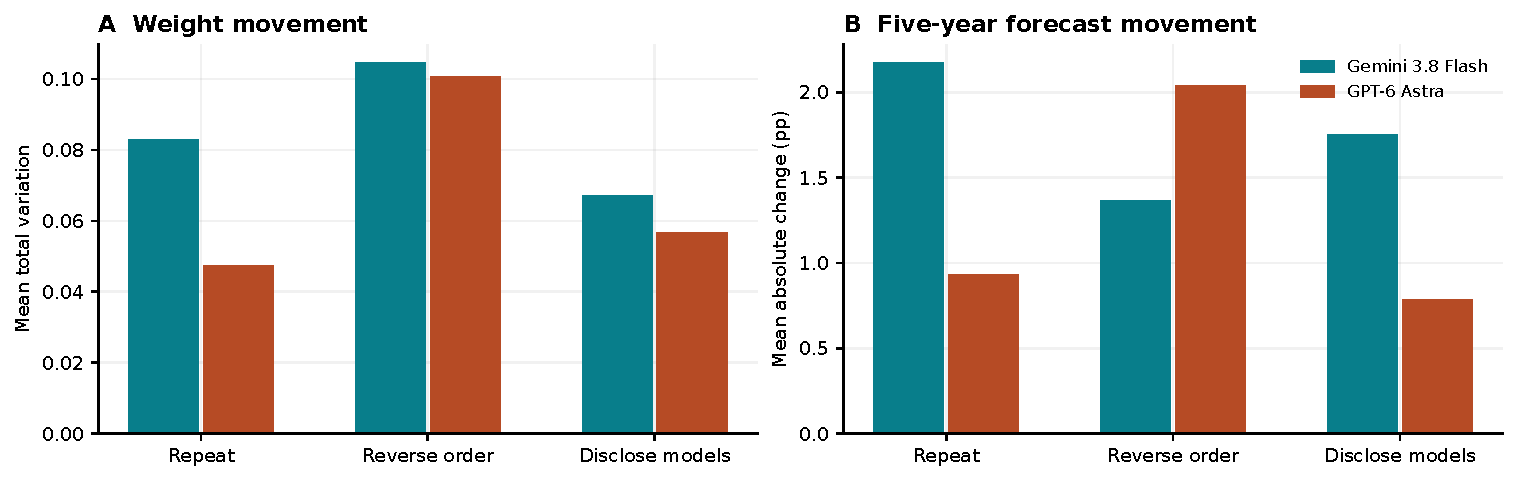
\includegraphics[width=\linewidth]{figures/stability.pdf}
\caption{Mean paired movement across six equities, relative to each synthesizer's original blinded baseline. Left: total variation of weights. Right: absolute five-year return difference. Each bar summarizes six deliberately selected assets and one paired realization per condition; it is not an estimate with a measured sampling error.}
\label{fig:stability}
\end{figure}

\subsection{The definition of consensus can change the sign}
The pooling operator is itself consequential. With Gemini's Nebius baseline weights fixed, quarter-by-quarter pooling produces $-0.42\%$, while averaging the completed source paths produces $+6.95\%$. For Moderna, the corresponding Gemini forecasts are $+4.98\%$ and $+15.03\%$, a 10.06-point gap. Astra's Moderna forecast changes from $-9.98\%$ to $-4.41\%$ under the same operator substitution.

This calculation requires no new language-model execution and changes neither evidence nor weights. It shows why a reproducible consensus release must specify the arithmetic, not merely publish a narrative about weighting. It does not prove that either operator is economically preferable. The choice should follow the intended forecasting target and be evaluated prospectively.

Normalization is another implementation detail worth exposing. Eighteen of 28 Gemini outputs require normalization of submitted scores; their submitted totals range from 1.00 to 1.40. All 28 Astra totals equal 1.00. The response contract permits normalization, so this is not evidence of eighteen invalid forecasts. It explains why submitted scores and final normalized allocations must both be retained.

\section{What this case study changes about an ensemble audit}
The practical lesson is to inspect the synthesizer as part of the model, rather than treating it as a neutral editor. Four records make that inspection possible: the source reports and their disagreement; the assigned influence; the numerical operator; and the resulting forecast under explicit perturbations. None is a substitute for the others.

First, an audit should preserve a blinded baseline and an unchanged-prompt repeat before interpreting a treatment difference. Here, that modest comparison changes the reading of the Opus result. Second, it should preserve report-level weights rather than only family totals. Twelve Gemini reports and one Astra report are different units of analysis, even when both are called a model family. Third, it should carry weight changes through the frozen forecast matrix. Visa and Bitcoin show why nearly unanimous direction is not enough to characterize numerical sensitivity. Fourth, it should publish the pooling operator and simple deterministic comparators alongside language-model synthesis.

These practices travel beyond financial research. A medical, legal, or scientific ensemble may also contain a final model that allocates credibility to competing reports. The present data do not establish effects in those domains; they illustrate what must be recorded to test them. Continuous influence and inspectable downstream calculations make it possible to distinguish disagreement that matters from disagreement that merely changes the wording of the summary.

\section{Limitations and prospective evaluation}
\textbf{Small, selected sample.} The six equities were selected to span agreement and dispersion, plus a fixed Bitcoin reference. The panel does not support population-level estimates, general vendor rankings, or inference based on treating the 784 weights as independent observations. The complete selection universe is not independently reconstructed.

\textbf{Unequal source composition and unknown quality.} Twelve reports share one source-model family. Framework diversity is not evidence of statistical independence. The Astra and Opus reports are not quality-matched controls. Evidence-link counts differ across source formats; missing structured links are not proof that a report used no research, and more links do not verify factual accuracy.

\textbf{Tools and timing.} Identical saved source reports do not guarantee identical information at synthesis time. Web access was enabled. The 28 new Astra receipts contain 166 web-search tool events, including different action types; these are not necessarily 166 distinct search queries. Only one of the 21 new Gemini receipts exposes grounded-response metadata, containing two queries. Missing metadata does not establish no retrieval. Provider differences confound model-only attribution, and the reused Gemini baselines are temporally separated from the experimental repeats.

\textbf{Limited replications and treatment purity.} One reverse ordering does not characterize arbitrary permutations. One disclosed realization does not estimate a disclosure-effect distribution. The two blinded runs provide a reference sensitivity check, not a reliable variance estimate. Bitcoin's additional checklist confounds its two treatment contrasts. Explicit-label blinding is incomplete protection against source recognition.

\textbf{Provenance boundaries.} All seven original Gemini request bodies were recovered and match their archived SHA-256 hashes. Numerical baseline payloads are available for all seven. Per-response provider receipts for all reused baselines are not fully recovered, so the incremental experiment resource table excludes those seven runs; recovered parent-release usage is accounted for separately. The released closure ledger reconciles successful logical tasks, not all retries or charges. Operational timestamps are not independent evidence of external preregistration.

\textbf{No outcome validation yet.} The first equity targets are 18 December 2026; Bitcoin's is 20 December 2026. No target has matured at the manuscript cutoff. Forecasts are point paths, not calibrated distributions, so neither source spread nor ensemble disagreement can be interpreted as predictive coverage. No profit, calibration, or return-superiority claim follows from the present analysis.

A future outcome study should fix its scoring rules, price sources, corporate-action treatment, market-calendar alignment, and missing-observation rules before examining realized targets. A natural baseline set includes the individual reports, equal-report and equal-model pooling, and both synthesizers. The fourth equity step falls on 18 September 2027, a Saturday, making the calendar rule material. We include a prospective evaluation specification in the companion materials, explicitly marked as proposed rather than registered. The present paper does not retrospectively choose a scoring rule after observing outcomes.

\section{Conclusion}
The same reports can yield a different forecast because a different model decides how much each report counts. In this archived panel, changing the synthesizer reverses two equity forecasts' five-year direction and shifts Bitcoin's projected return by 29.45 percentage points. Source disclosure selectively increases Astra's own-source influence across the six matched equities, while a blinded repeat weakens the interpretation of an Opus penalty. Neither result establishes predictive superiority or a causal self-preference mechanism.

The wider methodological point is that multi-agent consensus has an inspectable chain: reports, influence, arithmetic, and consequences. Evaluating only the final prose misses that chain. Recording it makes the ensemble's judgment testable now, and its accuracy testable when the future arrives.

\section*{Data, code, and disclosures}
The companion release contains 98 frozen source reports, 56 consensus outputs and request bodies, 784 allocations, 1,960 source-quarter and 1,120 consensus-quarter records, and offline reproduction code. It preserves the primary Gemini baselines, source configuration mappings, and completed-parent-release usage fields. The release includes seven archived anchors and 2,499 initial forecast-price points. Historical backgrounds use a separate retrospective database extract; its daily and weekly price CSVs are not redistributed. The paper and original research data are licensed under CC BY 4.0, and reproduction code under MIT; third-party material retains its own terms. \href{https://github.com/TheFutureEdge/research-when-models-judge-models}{The versioned GitHub repository} provides the replication files; the archival dataset identifier is \href{https://doi.org/10.5281/zenodo.23083356}{doi:10.5281/zenodo.23083356}.

The author is the founder of Future Edge Group FZE, which develops iPulse AI, and has a commercial interest in the platform studied. AI systems assisted with research operations, coding, audit, and manuscript preparation. Authorship and responsibility for the final submission remain with the named human author. The study reports system behavior rather than investment advice. Provider names identify archived source and synthesis configurations; they do not imply provider endorsement.

\begin{thebibliography}{99}\small
\bibitem{bates} J. M. Bates and C. W. J. Granger. The Combination of Forecasts. \emph{Operational Research Quarterly}, 20:451--468, 1969. \href{https://doi.org/10.1057/jors.1969.103}{doi:10.1057/jors.1969.103}.
\bibitem{blender} D. Jiang, X. Ren, and B. Y. Lin. LLM-Blender: Ensembling Large Language Models with Pairwise Ranking and Generative Fusion. \emph{ACL}, pp. 14165--14178, 2023. \href{https://aclanthology.org/2023.acl-long.792/}{doi:10.18653/v1/2023.acl-long.792}.
\bibitem{moa} J. Wang, J. Wang, B. Athiwaratkun, C. Zhang, and J. Zou. Mixture-of-Agents Enhances Large Language Model Capabilities. 2024. \href{https://arxiv.org/abs/2406.04692}{arXiv:2406.04692}.
\bibitem{selfmoa} W. Li, Y. Lin, M. Xia, and C. Jin. Rethinking Mixture-of-Agents: Is Mixing Different Large Language Models Beneficial? 2025. \href{https://arxiv.org/abs/2502.00674}{arXiv:2502.00674}.
\bibitem{mtbench} L. Zheng et al. Judging LLM-as-a-Judge with MT-Bench and Chatbot Arena. \emph{NeurIPS}, 2023. \href{https://arxiv.org/abs/2306.05685}{arXiv:2306.05685}.
\bibitem{panickssery} A. Panickssery, S. R. Bowman, and S. Feng. LLM Evaluators Recognize and Favor Their Own Generations. \emph{NeurIPS}, 2024. \href{https://arxiv.org/abs/2404.13076}{arXiv:2404.13076}.
\bibitem{wataoka} K. Wataoka, T. Takahashi, and R. Ri. Self-Preference Bias in LLM-as-a-Judge. 2024, revised 2025. \href{https://arxiv.org/abs/2410.21819}{arXiv:2410.21819}.
\bibitem{fair} P. Wang et al. Large Language Models are not Fair Evaluators. \emph{ACL}, 2024. \href{https://aclanthology.org/2024.acl-long.511/}{doi:10.18653/v1/2024.acl-long.511}.
\bibitem{sclar} M. Sclar, Y. Choi, Y. Tsvetkov, and A. Suhr. Quantifying Language Models' Sensitivity to Spurious Features in Prompt Design or: How I learned to start worrying about prompt formatting. \emph{ICLR}, 2024. \href{https://arxiv.org/abs/2310.11324}{arXiv:2310.11324}.
\bibitem{lostmiddle} N. F. Liu et al. Lost in the Middle: How Language Models Use Long Contexts. \emph{TACL}, 12:157--173, 2024. \href{https://aclanthology.org/2024.tacl-1.9/}{doi:10.1162/tacl\_a\_00638}.
\bibitem{turpin} M. Turpin, J. Michael, E. Perez, and S. R. Bowman. Language Models Don't Always Say What They Think: Unfaithful Explanations in Chain-of-Thought Prompting. \emph{NeurIPS}, 2023. \href{https://arxiv.org/abs/2305.04388}{arXiv:2305.04388}.
\bibitem{forecastbench} E. Karger et al. ForecastBench: A Dynamic Benchmark of AI Forecasting Capabilities. 2024, revised 2025. \href{https://arxiv.org/abs/2409.19839}{arXiv:2409.19839}.
\bibitem{gneiting} T. Gneiting. Making and Evaluating Point Forecasts. \emph{Journal of the American Statistical Association}, 106:746--762, 2011. \href{https://doi.org/10.1198/jasa.2011.r10138}{doi:10.1198/jasa.2011.r10138}.
\end{thebibliography}

\clearpage\appendix
\section{Historical context and all initial predictions}\label{app:history}
Each chart allocates half its width to five years of weekly-sampled BigQuery history and half to five years of forecasts. It shows the archived September anchor (white marker and vertical dotted line), all fourteen initial source paths (thin lines), both blinded consensus baselines, and equal-report quarter pooling. The shaded middle fifty percent describes opinion disagreement, not a probability interval. Prices use the original currency and anchor; no history is rescaled to fit a forecast. History is retrospective descriptive context, with the provenance limits stated in Section~\ref{sec:history}. The vertical scale differs by asset; compare disagreement quantitatively using Table~\ref{tab:initial} and Figure~\ref{fig:dispersion}.
\begin{figure}[H]
\centering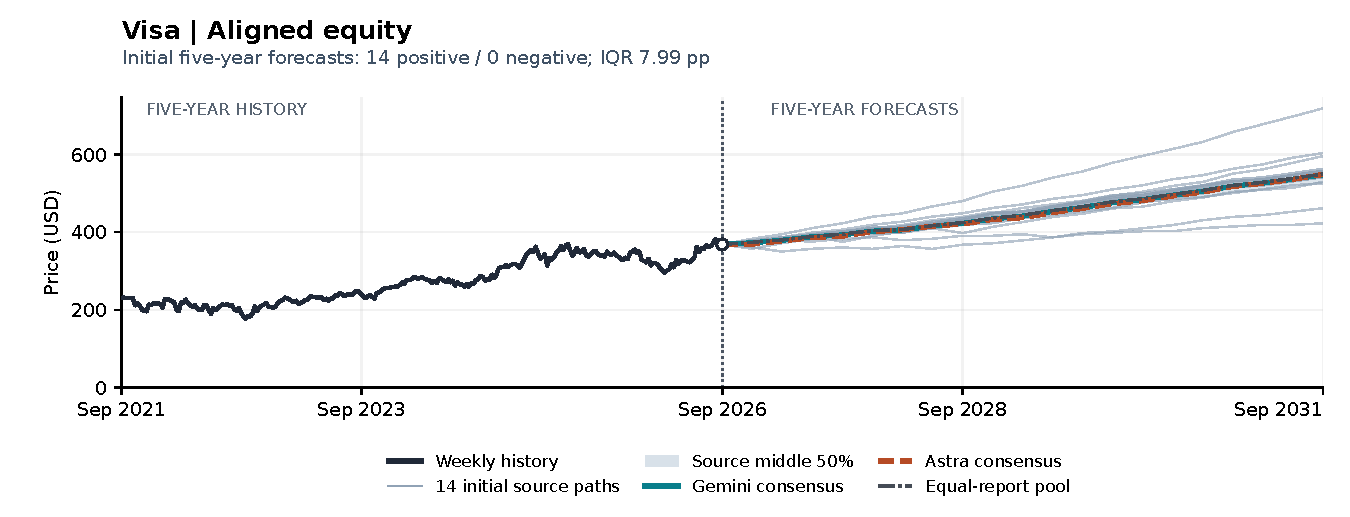
\includegraphics[width=\linewidth]{figures/history_forecast_visa.pdf}
\caption{Visa: aligned equity. All fourteen terminal predictions are positive, with a 7.99-point IQR. The consensus paths nearly overlap despite different allocations of influence. History: weekly last-observed BigQuery closes.}
\end{figure}
\begin{figure}[H]
\centering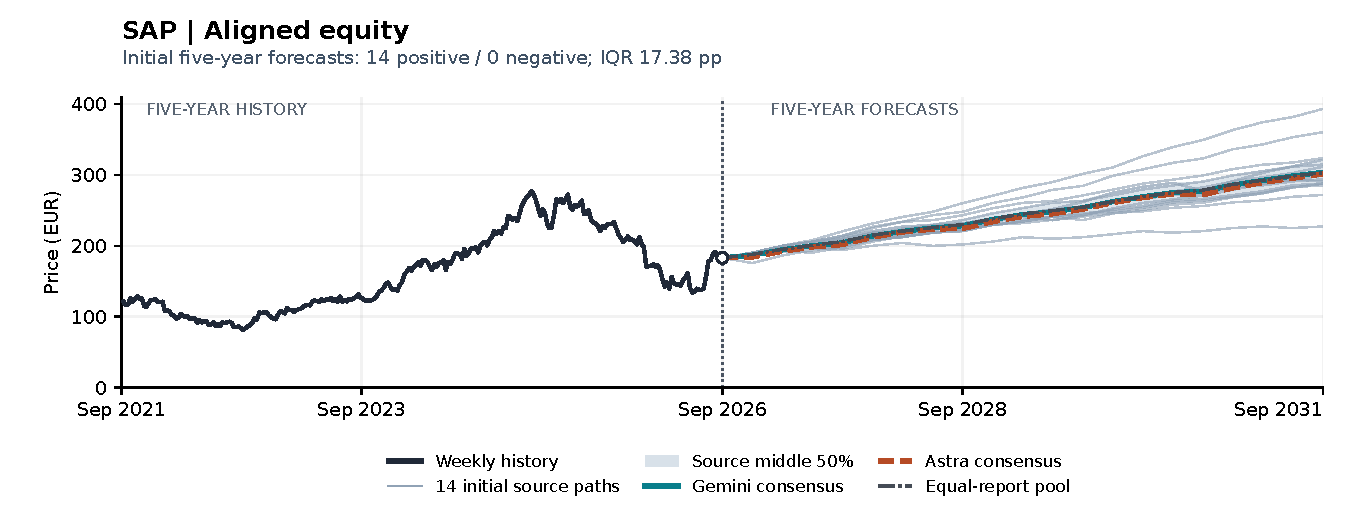
\includegraphics[width=\linewidth]{figures/history_forecast_sap.pdf}
\caption{SAP: aligned equity. The Xetra ordinary share is plotted in euros. All fourteen terminal predictions are positive; IQR is 17.38 points. History: weekly last-observed BigQuery closes.}
\end{figure}
\clearpage
\begin{figure}[H]
\centering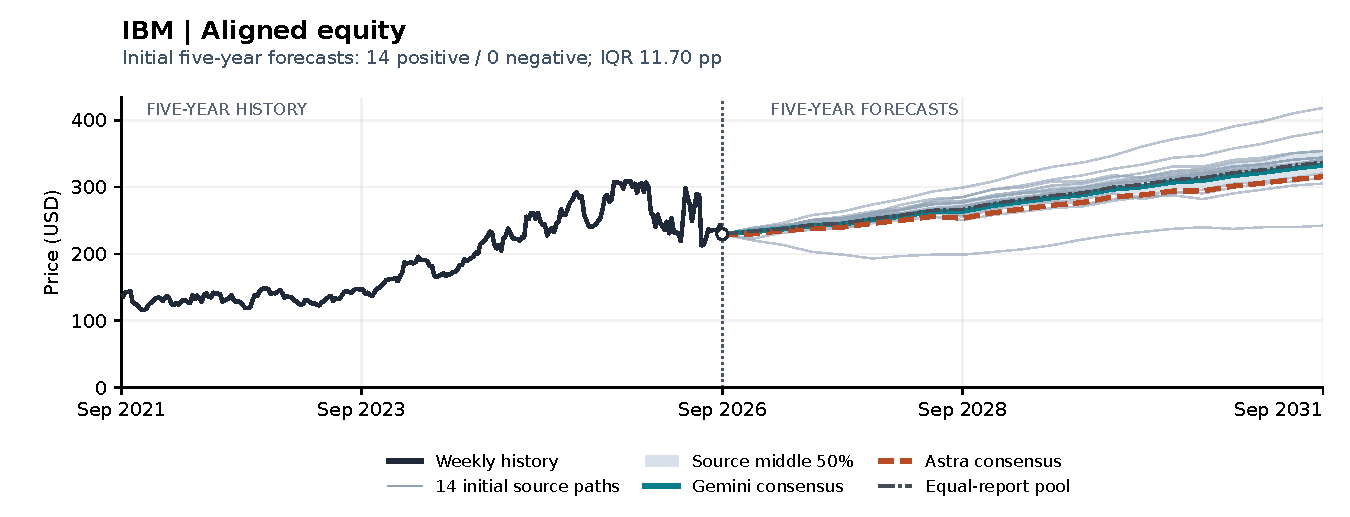
\includegraphics[width=\linewidth]{figures/history_forecast_ibm.pdf}
\caption{IBM: aligned equity. Unanimous positive terminal direction and an 11.70-point IQR coexist with a 7.53-point difference between consensus baselines. History: weekly last-observed BigQuery closes.}
\end{figure}
\begin{figure}[H]
\centering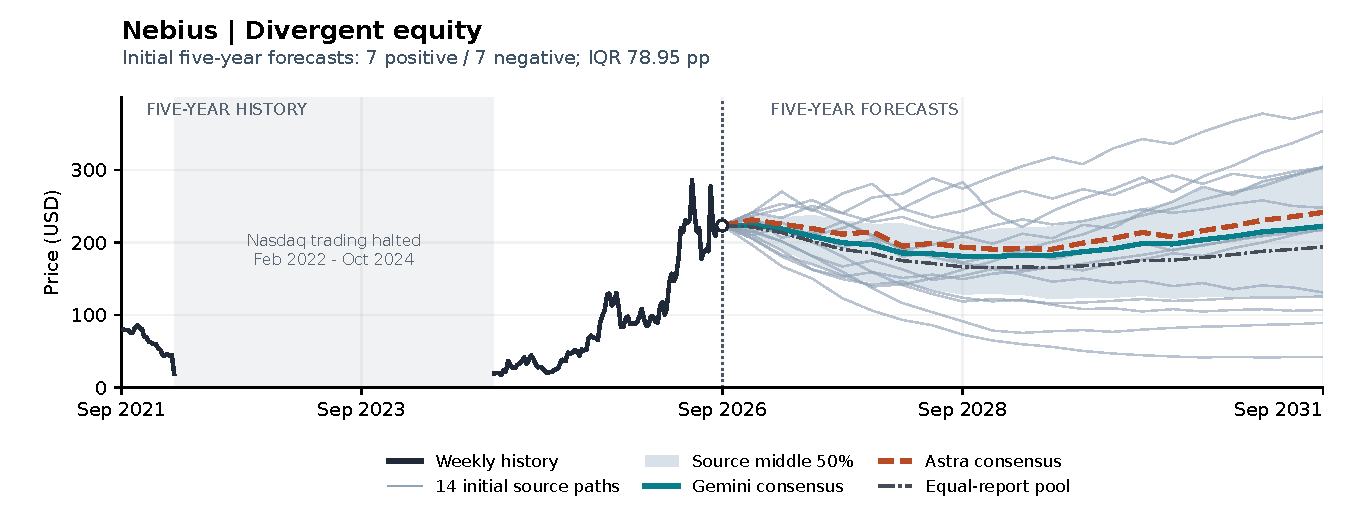
\includegraphics[width=\linewidth]{figures/history_forecast_nebius.pdf}
\caption{Nebius: divergent equity. Seven initial reports predict a positive terminal return and seven a negative return. Gemini's five-year consensus is $-0.42\%$; Astra's is $+8.10\%$. Earlier observations belong to the Yandex predecessor. The shaded gap marks the Nasdaq trading suspension from 28 February 2022 to 21 October 2024; it does not imply continuous trading. The company's \href{https://nebius.com/newsroom/nebius-group-n-v-announces-official-name-change-and-new-ticker-symbol}{name-change notice} and \href{https://nebius.com/newsroom/nebius-group-confirms-schedule-for-resumption-of-trading-on-nasdaq}{trading-resumption notice} document the transition.}
\end{figure}
\clearpage
\begin{figure}[H]
\centering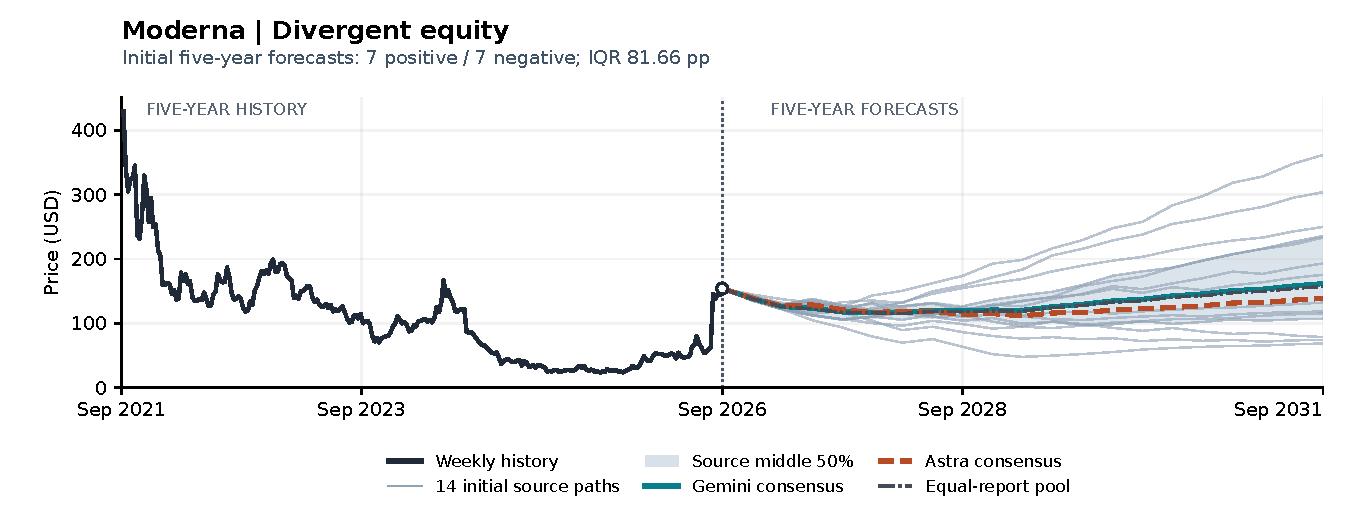
\includegraphics[width=\linewidth]{figures/history_forecast_moderna.pdf}
\caption{Moderna: divergent equity. The seven--seven directional split produces a broad fan of initial forecasts. The two consensus baselines end on opposite sides of the anchor, at $+4.98\%$ and $-9.98\%$. History: weekly last-observed BigQuery closes.}
\end{figure}
\begin{figure}[H]
\centering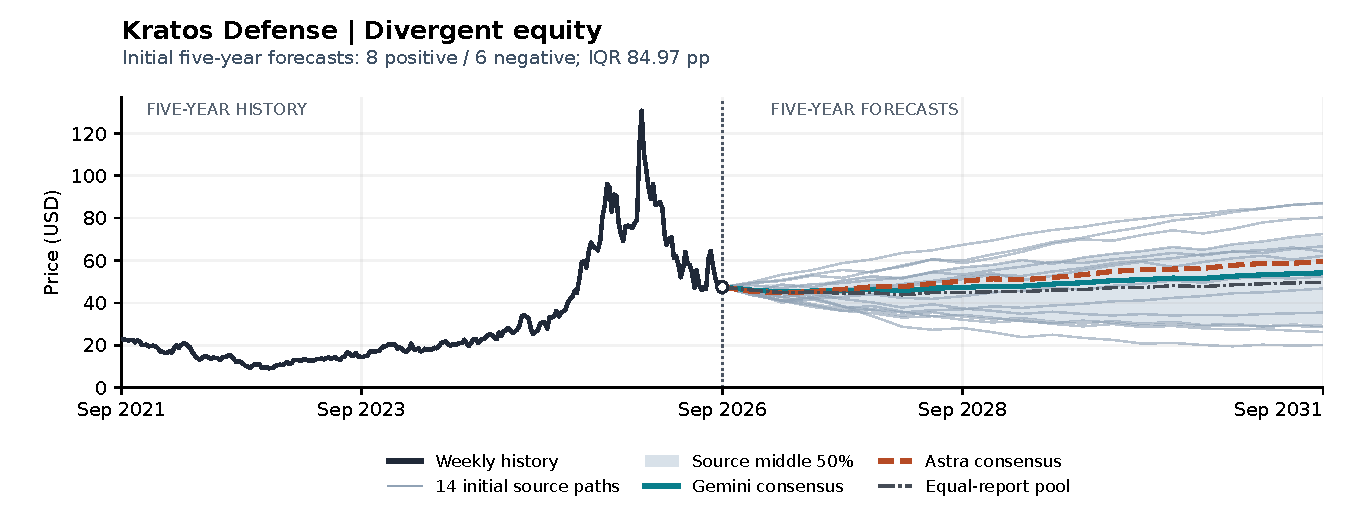
\includegraphics[width=\linewidth]{figures/history_forecast_kratos.pdf}
\caption{Kratos: divergent equity. Eight positive and six negative terminal predictions give the panel's widest terminal IQR, 84.97 points. Both consensuses are positive at five years, but differ by 11.45 points. History: weekly last-observed BigQuery closes.}
\end{figure}
\clearpage
\begin{figure}[H]
\centering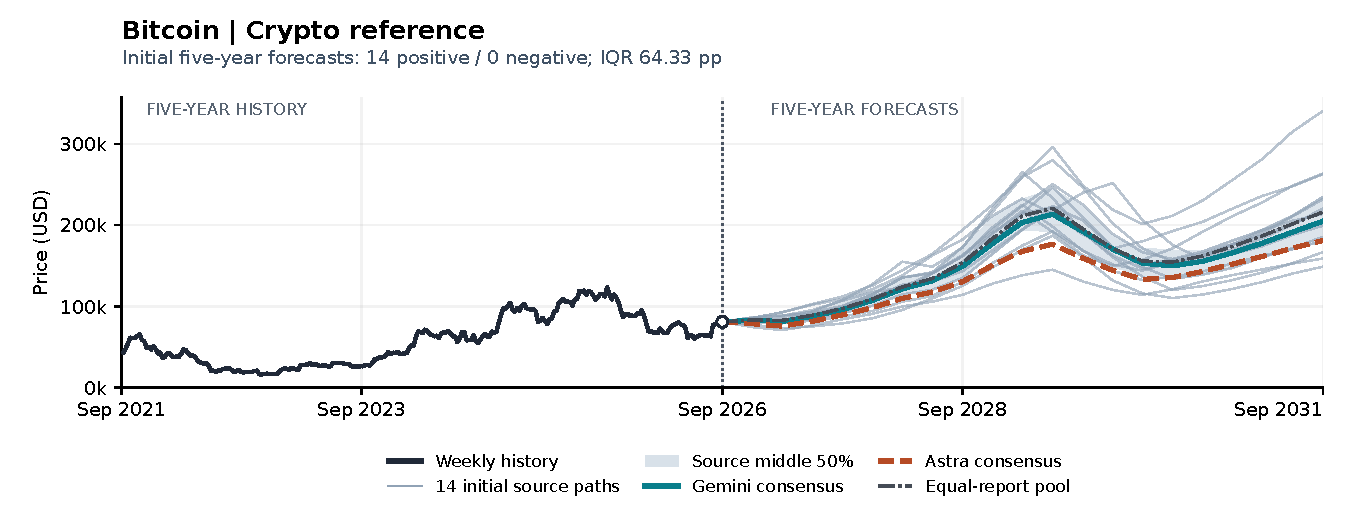
\includegraphics[width=\linewidth]{figures/history_forecast_bitcoin.pdf}
\caption{Bitcoin: separate crypto reference. All fourteen terminal predictions are positive, but the 64.33-point source IQR and 29.45-point consensus gap show substantial disagreement about magnitude. The paths also expose an intermediate rise, retreat and renewed increase that a terminal-return table hides. History: weekly BigQuery closes; the anchor retains the archived 20 September 2026 00:00 UTC reference.}
\label{fig:bitcoinhistory}
\end{figure}

These charts preserve the initial predictions irrespective of their eventual synthesis weights. The history and the forecast portions have different evidential roles: history locates the archived starting point, while the forward paths expose the alternatives from which each synthesizer constructs a consensus. The history does not validate those alternatives, and none of the forward curves is a realized outcome. The separate normalized seven-panel overview remains available among the companion figures for cross-asset inspection.
\clearpage

\section{Detailed robustness and numerical checks}
\begin{table}[ht]
\centering\small
\begin{tabular}{@{}llrrr@{}}
\toprule
Synthesizer & Comparison & Weight TV & One-year movement & Five-year movement \\
\midrule
Gemini & Same-order repeat & 0.0830 & 0.67 & 2.17 \\
Astra & Same-order repeat & 0.0475 & 0.29 & 0.93 \\
Gemini & Reverse order & 0.1045 & 0.57 & 1.37 \\
Astra & Reverse order & 0.1008 & 0.41 & 2.04 \\
Gemini & Model disclosed & 0.0671 & 0.33 & 1.75 \\
Astra & Model disclosed & 0.0567 & 0.25 & 0.79 \\
\bottomrule
\end{tabular}
\caption{Six-equity means relative to the original blinded baseline. Horizon movements are absolute cumulative-return differences in percentage points. Bitcoin is excluded because of the treatment-wrapper difference.}
\end{table}

\subsection{Sensitivity across the full path}
For a small weight perturbation $\delta w$ satisfying $\sum_i\delta w_i=0$, the first-order terminal change is
\begin{equation}
\delta R_T\approx (1+R_T(w))\sum_i\delta w_i\sum_{t=1}^{T}\frac{r_{it}}{1+q_t(w)}.
\end{equation}
This follows by differentiating Equation~\ref{eq:step}. It highlights two features: the effect depends on \emph{which} report gains weight, and it depends on that report's entire sequence of quarterly returns. It is a local approximation, not a replacement for exact recomputation at the observed weight vectors. The companion code uses exact compounding for all reported results and verifies the quarterly bound in Equation~\ref{eq:bound} for every paired treatment.

\subsection{Validation and reproducibility}
The supplied archival audit was rerun and passed 1,059 checks, including original file hashes, source identity counts, numerical paths, and comparison metrics. A separately implemented, standard-library reproduction passed 392 checks on the release's canonical inputs, including weight membership and normalization, all twenty quarterly returns, cumulative returns, forecast prices, and the per-quarter perturbation bound. These counts describe executable assertions, not independent experiments or external peer review.

The release provides both full JSON objects and tabular extracts. Numeric claims can be recomputed without network access, model credentials, a database, or the production application. Figure generation requires NumPy and Matplotlib; numerical reproduction itself uses only the Python standard library. Hash manifests identify the exact release files. The recovered baseline requests are checked against the hashes saved in the original experiment snapshots.

The archive also contains written justifications for every allocation. These make the system's stated reasons inspectable, but the present analysis does not code narrative quality, validate every cited source, or treat a generated justification as causal evidence of the model's internal reasoning.

\clearpage
\section{Resource accounting and evidence boundaries}\label{app:resources}
\subsection{The completed parent Batch 7 release}
Read-only production telemetry was recovered on 1 October 2026. Each of the 5,964 source task identifiers was hashed and matched to the archived closure ledger; the 426 completed consensus rows were matched to its asset symbols. Every source task has recorded usage. All fourteen framework/model/mode recipes occur for each of the 426 assets. Opus uses two recorded stages per source report (research and forecast), whereas the other source configurations and the consensus layer each contribute one recorded stage. Thus 6,390 logical tasks correspond to 6,816 recorded successful generation stages.

\begin{table}[H]
\centering\small
\begin{tabular}{@{}lrrrr@{}}
\toprule
Layer / model & Tasks & Stages & Input tokens & Generated tokens \\
\midrule
Source / Gemini & 5,112 & 5,112 & 401,410,457 & 119,731,864 \\
Source / Opus & 426 & 852 & 160,086,835 & 9,170,112 \\
Source / Astra & 426 & 426 & 38,020,284 & 7,279,753 \\
Consensus / Gemini & 426 & 426 & 43,776,810 & 5,001,248 \\
\midrule
Completed release & 6,390 & 6,816 & 643,294,386 & 141,182,977 \\
\bottomrule
\end{tabular}
\caption{Completed-release usage, including intermediate research stages and reasoning. Generated tokens comprise 38,620,594 non-reasoning output tokens and 102,562,383 reasoning tokens. Combined input and generated volume is 784,477,363 provider-defined tokens. Raw usage fields, hashed task identifiers, normalization rules, and offline reconciliation code accompany the paper.}
\label{tab:parentusage}
\end{table}

This is a \emph{completed-release footprint}, not an all-attempts or billing total. It excludes failed and superseded attempts, preview syntheses, and the 49 additional experiment requests below. Reused Gemini experiment baselines already belong to the parent release and must not be counted again. Input totals include cached and repeatedly supplied context, including intermediate research when it is passed into a later stage. They are not counts of unique documents, words read, or new knowledge. Provider tokenizers differ; these totals do not establish comparable compute, efficiency, or forecast quality.

For Gemini, generated tokens are candidate plus thought tokens; cached input is already part of prompt tokens. For Opus, input sums ordinary input, cache creation, and cache reads; thinking is already included in output. Astra's recorded output likewise includes reasoning. Normalization follows the provider usage fields and checks exact arithmetic where total fields are available. The release records links to the provider documentation and preserves the original usage dictionaries.

\clearpage
\subsection{Incremental synthesis experiment}
\begin{table}[H]
\centering\small
\begin{tabular}{@{}lrr@{}}
\toprule
Recorded quantity & Gemini, 21 new runs & Astra, 28 new runs \\
\midrule
Input tokens & 2,163,764 & 4,072,549 \\
Candidate/output tokens & 140,376 & 496,597 \\
Thinking/reasoning tokens & 110,203 & 317,893 \\
Cached input tokens & 92,611 & 803,409 \\
Recorded total tokens & 2,414,343 & 4,569,146 \\
\bottomrule
\end{tabular}
\caption{Provider-recorded resource totals for new experimental requests only. Astra reasoning tokens are included in output tokens; Gemini thinking tokens are separately reported and included in total tokens. Cached tokens are a subset of input, not additional usage. The columns have different numbers of requests and provider accounting conventions.}
\end{table}

No dollar-cost estimate is inferred from current list prices. Complete billed cost requires the applicable historical pricing, discounts, search charges, and missing reused-baseline receipts. These token totals cannot establish that one synthesizer is more cost-effective: the experiment neither equalizes compute nor measures matured forecast skill.

The parent ledger, source snapshots, request hashes, and provider receipts answer different provenance questions. A ledger can reconcile successful task counts without proving every raw provider response. A request hash can establish content equality without proving exactly what external retrieval returned. We preserve those distinctions in the release's evidence inventory rather than collapsing them into a single claim of complete end-to-end reproducibility.

\end{document}
